\section{Interferenza}
Per analizzare il fenomeno dell'interferenza abbiamo predisposto l'apparato differentemente per due diverse esperienze.

\subsection{Esperienza di Michelson}
In primis abbiamo disposto le lenti e gli specchi come riportato in Figura \ref{michelino}

\begin{figure}[h!]
    \centering
    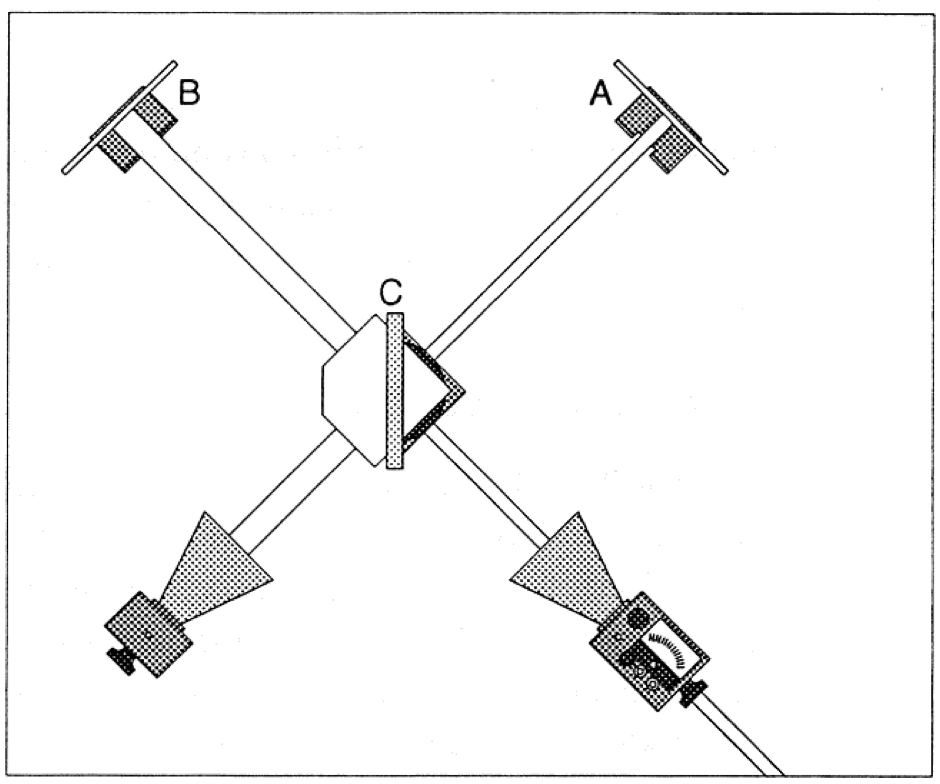
\includegraphics[scale=.35]{Immagini/michelino.png}
    \caption{Configurazione di Michelson}
    \label{michelino}
\end{figure}
\noindent
Mantenendo tutte le componenti fisse, abbiamo proceduto spostando una delle lastre semi-riflettenti con intervalli di $\Delta d = 10 cm$. Dopo aver contato il numero di massimi per tale spostamento, abbiamo calcolato la relativa lunghezza d'onda $\lambda$, utilizzando la seguente relazione:

\begin{equation}
    \lambda=2\dfrac{L_{M1} + \Delta d - L_f}{\Delta N}
\end{equation}
dove $L_{M1}$ indica la posizione iniziale dello specchio mobile e $L_F$ indica la posizione iniziale dello specchio fisso
\noindent
Riportiamo di seguito i valori ricavati:

\begin{table}[h!]
    \centering
    \begin{tabular}{c|cc}
    Numero di massimi & $\lambda$ $(cm)$ & $\sigma_\lambda$ ($cm$)\\
    \hline
6	&	3,33	&0,06\\
6	&	3,33	&0,06\\
7	&	2,86	&0,05\\
7	&	2,86	&0,05\\
7	&	2,86	&0,05\\
7	&	2,86	&0,05\\
7	&	2,86	&0,05\\
7	&	2,86	&0,05\\
8	&	2,50	&0,04\\
7&		2,86&	0,05\\
6	&	3,33	&0,06\\
6&		3,33&	0,06\\
7&		2,86&	0,05\\
7	&	2,86	&0,05\\
7	&	2,86	&0,05\\
7	&	2,86	&0,05\\
7	&	2,86	&0,05\\
\hline\hline
    \end{tabular}
    \caption{Caption}
    \label{tab:my_label}
\end{table}
\noindent
Il valore medio della lunghezza d'onda e il relativo errore, calcolato come media di ogni errore calcolato con il metodo della propagazione degli errori, è di 
$$
\lambda = 2,948 \pm 0,051\, cm
$$
\subsection{Esperienza di Lloyd}
Anche il questo caso lo scopo dell'esperimento è stato quello di determinare la lunghezza d'onda attraverso lo studio del fenomeno dell'interferenza.

Predisposte le componenti come in Figura \ref{loyd} abbiamo cercato di rilevare la posizione dei massimi a partire dal primo. Tale operazione è risultata difficile a causa delle numerose fonti d'incertezze. 

\begin{figure}[h!]
    \centering
    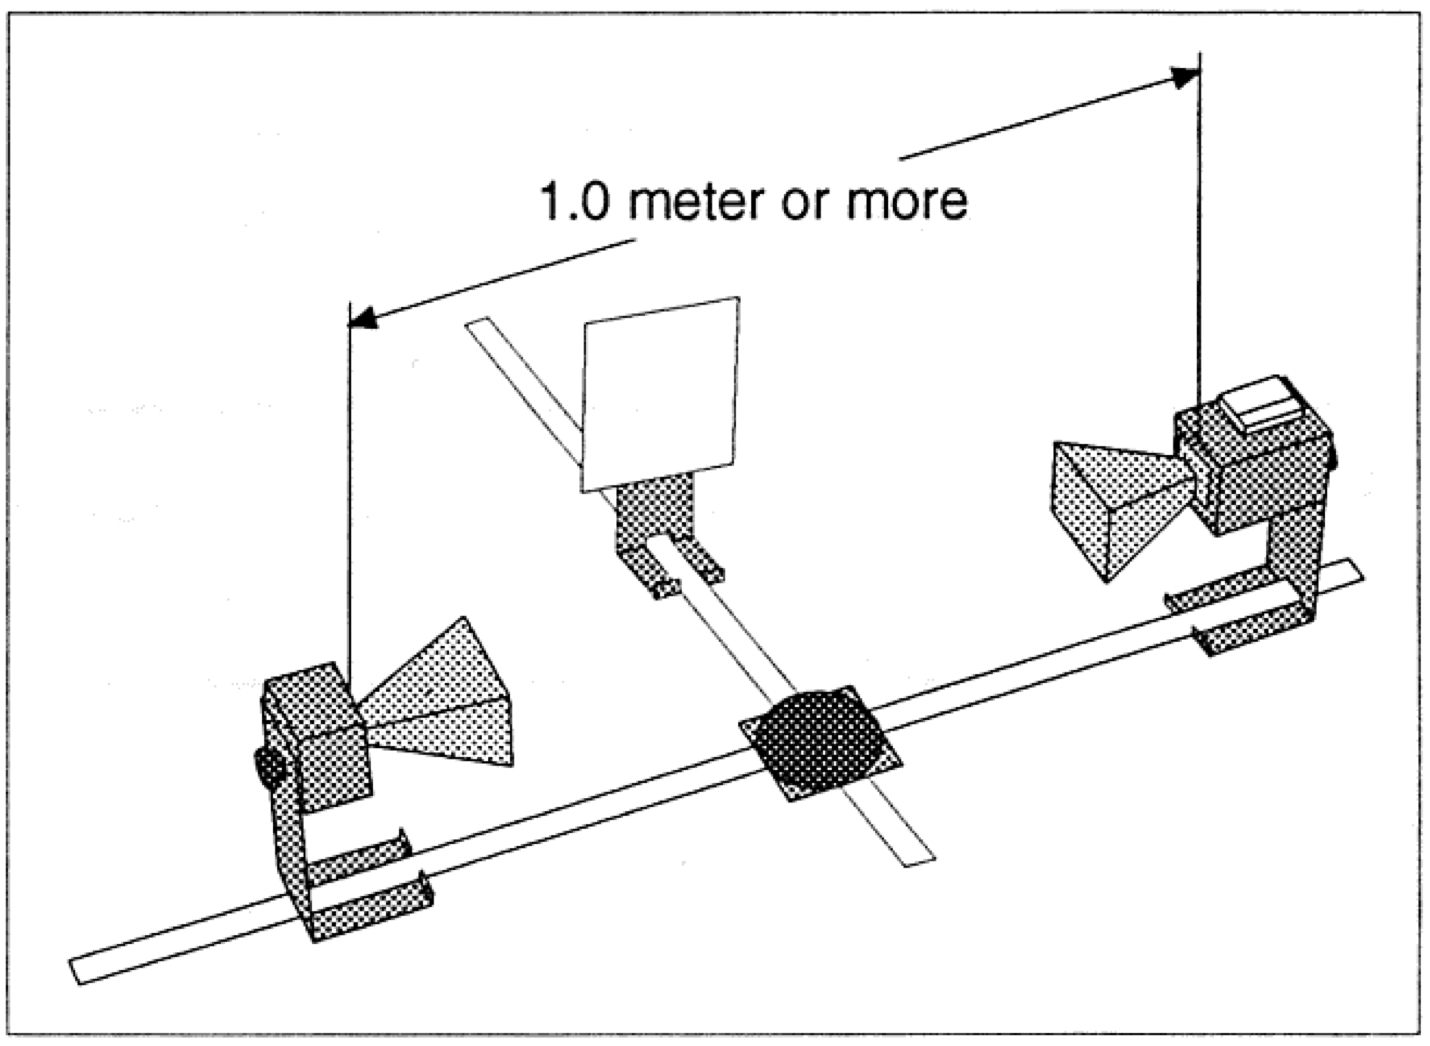
\includegraphics[scale=.35]{Immagini/loid.png}
    \caption{}
    \label{loyd}
\end{figure}
\noindent
I dati raccolti sono i seguenti:
\begin{table}[h!]
    \centering
    \begin{tabular}{ccc}
        Numero del massimo & $d$ $(cm)$ & $\lambda$ $(cm)$ \\
        \hline 
    1&	3,4&1,0	\\
    2&	4,4&5,1	\\
    3&	9,5&2,5	\\
    4&	12&	   4,0 \\
    5&	16&	    8,1\\
    6&	24,1&	\\
\hline\hline
\end{tabular}
\end{table}

E' ben visibile l'errore che traspare dalle misurazioni effettuate, esso verrà discusso nel dettaglio all'interno delle conclusioni.
